%\addcontentsline{toc}{subsection}{Note on the available R package : \texttt{evdbayes}}
\section{Available Methods : \texttt{evdbayes}}

The \texttt{evdbayes} package is the only available on CRAN to do Bayesian inference in EVT with MCMC techniques to sample from the posterior (see \citet{ribatet_users_2006}), which is a very old package. We have passed a long time trying to understand and compute relevant analysis with the \texttt{evdbayes} framework. We had problems to understand both its structure and the famous "black-box".
 Since we faced important problems, e.g. it was impossible to reach the stationary posterior distribution of our of the parameter $\mu_1$ in a nonstationary GEV analysis with linear trend on $\mu(t)$, we decided to develop our own methods. Moreover, following \citet{hartmann_bayesian_2016}, it only uses the Metropolis Hastings (MH) Algorithm \ref{algo:mh} (\hyperref[app:algo]{Appendix \textbf{\ref{app:algo}}}) which is quite restrictive. We then decided to develop not only the MH but also the Gibbs sampler, and later the Hamiltonian Monte Carlo through the STAN interface. 

The different methods to compute the prior $\pi(\theta)$ discussed in \hyperref[sec:prior]{Section \textbf{\ref{sec:prior}}} are available in the \texttt{evdbayes} package. Since we mostly rely on our functions and we have no experts' advices, we will rather use vague priors (see \hyperref[sec:noninfoprior]{Section \textbf{\ref{sec:noninfoprior}}}. 


 Note that efforts should put to the new \texttt{revdbayes} R package which use the generalised ratio-of-uniforms method instead of the popular MCMC techniques, which is an other acceptance-rejection type of simulation algorithm. ( \hyperref[sec:bayes_ratio]{Section \textbf{\ref{sec:bayes_ratio}}}) ? )
 
 
 
 We have considered several methods : 
 
 \begin{itemize}
 	\item evdbayes package
 	\item From Our Functions (R package)
 	\item Ratio of Uniform : \texttt{revdbayes} package :
 	
 	\url{https://cran.r-project.org/web/packages/revdbayes/vignettes/revdbayes-vignette.html}
 	
 	Helped with \texttt{rust}
 	
 	\item From HMC algorithm using STAN language :
 	
 	The problem is maybe from \ref{likgevintro}. The parameter $\xi$ is relatively near the region that could be problematic, causing convergence issues. 
 	
 \end{itemize}
%\section{From Our Functions (R package)}

The methods we have computed for the MH algorithm and the Gibbs sampler are based on Algorithm \ref{algo:mh} and Algorithm \ref{algo:gib}.

\section{Stationary GEV}

Note that the results for the stationary model are very similar to those obtained with \texttt{evdbayes}. We empirically verify that the latter rather uses the MH algorithm.

\subsection*{Comparison Metropolis-Hastings and Gibbs Sampler}



\paragraph{Gibbs Sampler}

This is done by tuning the standard deviation $\sigma^{(j)}$ of the proposal $p_{t,j}\big(\theta_*^{(j)}|\theta_{t-1}^{(j)}\big)$. Although the $\theta^{(j)}$ are taken to be univariate in our case, it is difficult to tune each $\sigma^{(j)}$ to achieve average acceptance probabilities for all parameters. We will then use a \emph{trial-and-error} approach.


\section{Nonstationary GEV}


To limit the influence of the (randomly) selected starting values, we take a burn-in period of length $B=N/....$ 
This is probably too conservative, but it is relatively fast in our example (?) and therefore it is not much important.


\subsection{Model Comparisons}




We willl compare the same parametric models as in \hyperref[sec:xpnp]{Section \textbf{\ref{sec:xpnp}}} but with Bayesian techniques coming from \hyperref[sec:modcompbay]{Section \textbf{\ref{sec:modcompbay}}}. It will be interesting to see whether there are differences in the selected model between the frequentist and the Bayesian frameworks.

 



\subsection{Posterior Predictive Distribution} 

 \begin{figure}[!htb]
  	\centering	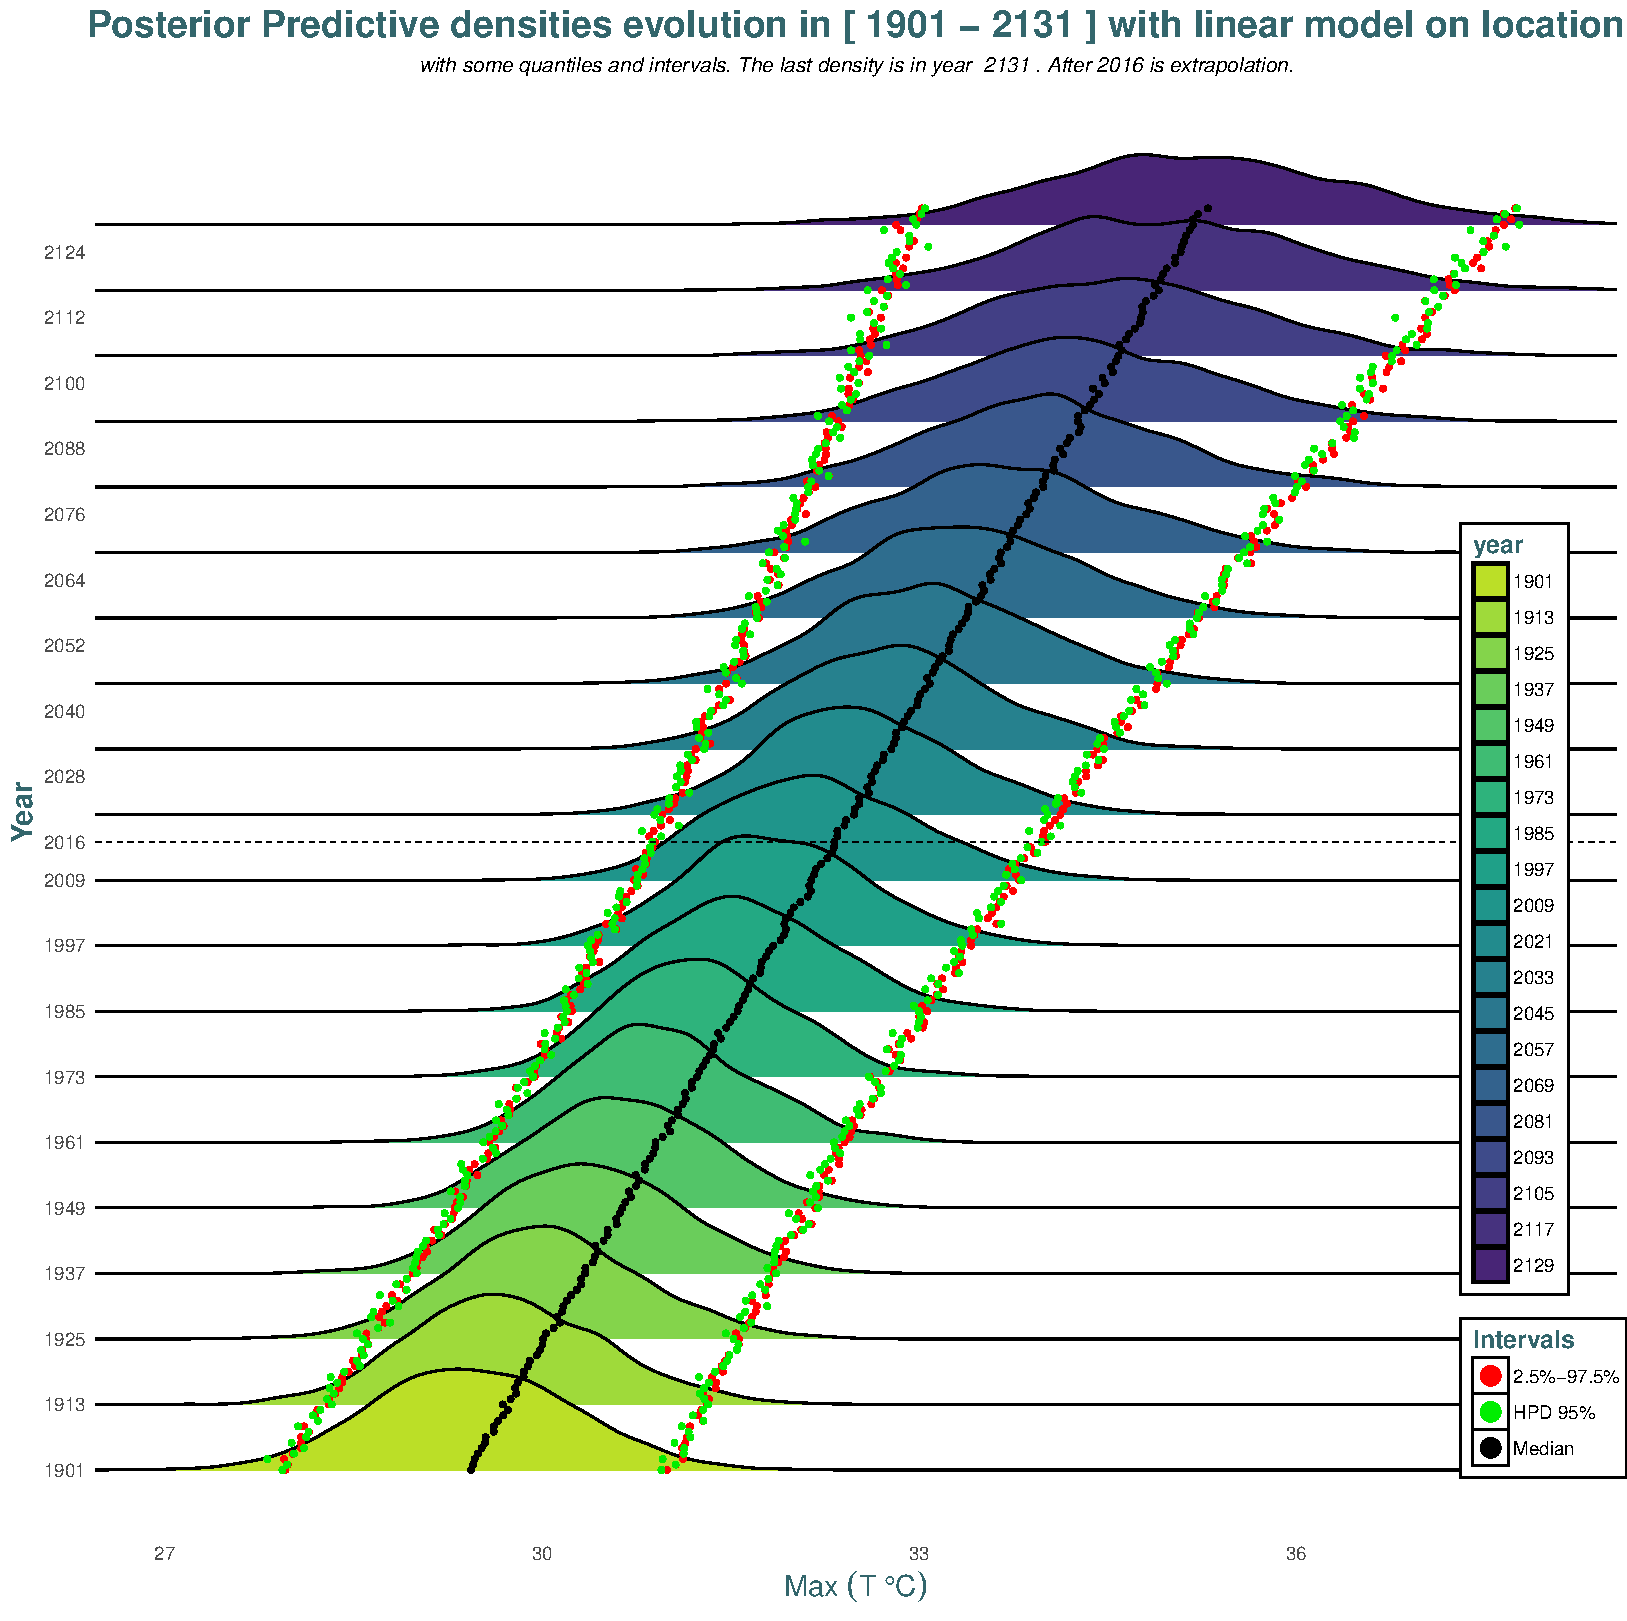
\includegraphics[width=0.8\linewidth]{predpred.pdf}\caption{ }\label{fig:post_pred}
 \end{figure}
  
  
  We remark from this graph the increasing variance of the predictive posterior as far as we predict in the future. It can also be seen from the $5\%$ and $95\%$ quantiles which deviate from the median. 
  
%\section{From HMC algorithm using STAN language}
%\section{Ratio of Uniform : \texttt{revdbayes} package}\label{sec:bayes_ratio}


\subsubsection*{Predictive Information Criteria}

For each generated chains with dispersed starting values, we evaluate separately the information criteria. The discrepancies between the chains are small (?), which is a good sign. 


\subsection{Diagnostics}


From the autocorrelation, we calculate the effective sample size () The effective sample size $N_{eff}$ (\ref{eq:neff}) is 

\subsubsection*{Sensitivity Analysis}

\textbf{section 7.4} evdbayes pdf + suppplément risk book 

The basic sensitivity analysis works by fitting several models to
the same problem. Posterior inferences can then be compared.
The sensitivity of the
marginal posterior density of the shape parameter $\xi$ is often of particular interest.


The basic method of sensitivity analysis is to fit several models to the same problem.
 Posterior inferences from each model can then be compared. Posterior inferences
will typically include marginal posterior distributions of the 3 parameters posterior distributions of GEV quantiles and posterior predictive distributions.
The sensitivity of the marginal posterior density of the shape parameter $\xi$ is often of particular interest.



\section{Comparisons}

\citet{hartmann_bayesian_2016}
We can calculate the effective sample size (ESS) using the posterior samples for each parameter : 

\begin{equation}
\text{ESS}=N\cdot (1+2\sum_k\gamma(k))^{-1}
\end{equation}

where $N$ is still the number of posterior samples and $\gamma(k)$ are the monotone lag $k$ sample autocorrelations. \citet{geyer__1992}. We can thus interpret this as the number of effectively independent samples. 


\subsection{STAN}

Benefits : 

\begin{itemize}
	\item Allows more flexibility (?) through the mathematical formulation of the formula
	\item It is really smoother and clearer (straightforward) for this kind of problems 
\end{itemize}

Drawbacks : 

\begin{itemize}
	\item New language with all the problems/errors arising when learning it. 
\end{itemize}



"for time critical operations it may be nec-
essary to use a compiled language either in preference to R or as a subroutine that
is called from R. In our experience this typically results in a two-fold or three-fold
speed increase over optimized R code for iterative simulation algorithms of the type
used in Markov chain Monte Carlo simulation."

\section{Comparison with frequentists results}

In this first analysis, we rely on 


By using objective priors (i.e. priors with very large variance), we should obtain the same results in the frequentist or in the Bayesian setting, which will be a prove of robustness of obtained results  
